\chapter{Requirements}

See appendix ~\ref{appendix:requirements} for my Cucumber features.


\section{Use cases}

Having clarified what the requirements of the system were through my feature files, I created numerous use-case diagrams to visualise this information. By doing so, I hoped to be able to derive classes and functionalities by examining similar or duplicating use case scenarios. I first turned my attention to user registration.

\subsection{Registration}

\begin{figure}[h!]
  \centering
    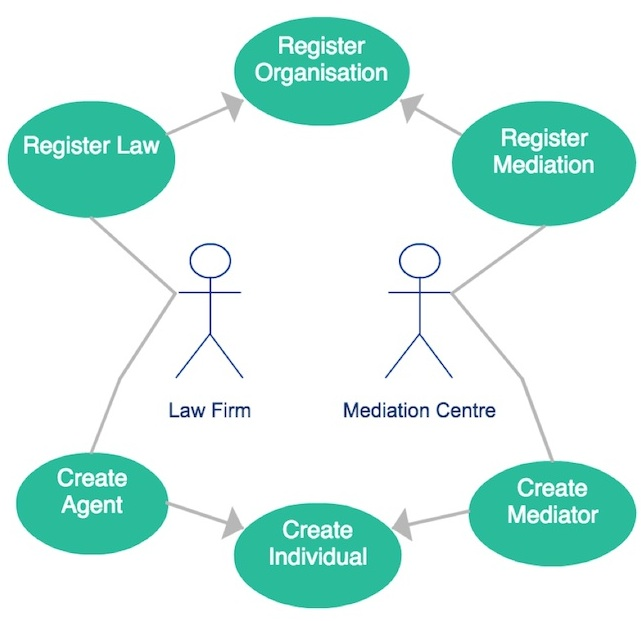
\includegraphics{use_case--registration}
  \caption{Use case diagram showing registration feature}
  \label{uml:useCase:registration}
\end{figure}

We know that authorised individuals should be allowed to register accounts representing their company (be it a law firm or mediation centre), and that within that organised account they should be able to register individual accounts, which should be agents or mediators depending on the organisation type.

Figure ~\ref{uml:useCase:registration} shows this in terms of the law firms and mediation centres. In both the organisational and individual registration, I've added a generalised action that the specialised registrations can extend or implement, showing where I might be able to use a common class or database table to accomplish both goals.

\subsection{Disputes}

\begin{figure}[h!]
  \centering
    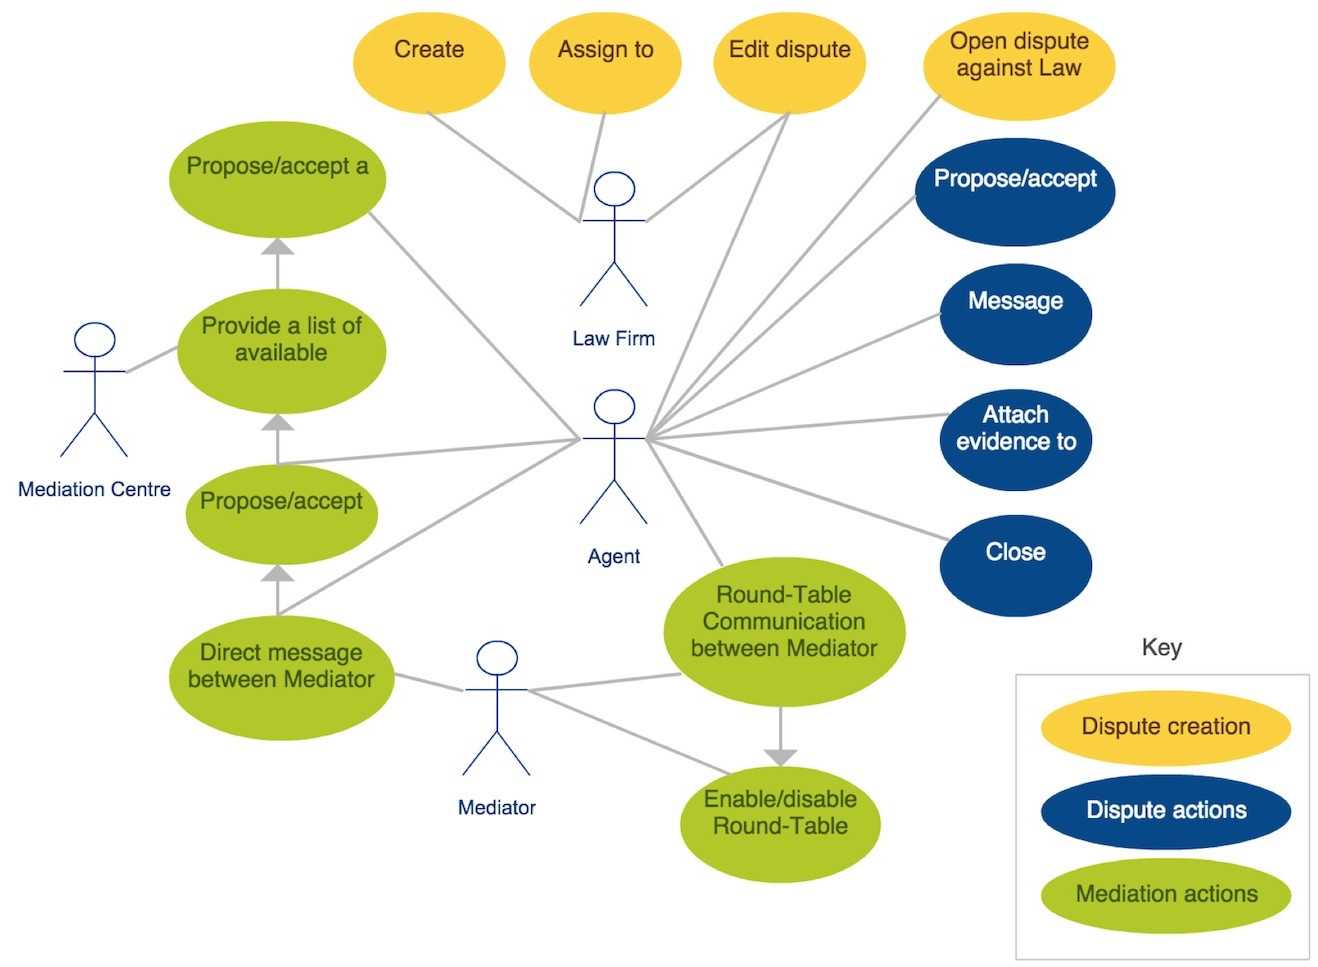
\includegraphics[width=\textwidth]{use_case--disputes}
  \caption{Use case diagram showing actions available in a dispute}
  \label{uml:useCase:disputes}
\end{figure}

Only law firms can create new disputes. There is then some back-and-forth assignment between law firms and agents until both sides of a dispute are represented by different agents. I identified this as being a "dispute creation" stage.

Inside a dispute, agents should be able to negotiate the dispute lifespan, exchange messages and evidence, and should have the freedom to close a dispute. In a best-case scenario, this is all that is required to successfully resolve a dispute. I've identified this as the "dispute" stage.

Should it be required, an agent can propose mediation, and there is a defined process of administration between the agents and mediation centre required to get the dispute "into mediation". Once in this state, the agents can communicate only through the mediator, unless the mediator feels the dispute is close to resolution and decides to enable round-table communication.

\subsection{Miscellaneous}

Other elements of functionality are implied in the feature files. For example, agents should be able to peruse a mediator's CV before making a decision as to which mediator to opt for. This suggests a "view profile" facility, with custom fields for the CV, which could be as simple as a HTML textarea or as complicated as an integrated PDF uploader and viewer.

Given the tight deadline of the project, the scale of the system I'll be building, and the priority having to be on the maritime collision logic, I was told to keep these miscellaneous features as simple as possible.

